\lecture{绪论}{lec:chap02}
\section[知识回顾]{知识回顾}\label{sec:chap02-sec00}
%%%%%%%%%%%%%%%%%%%%%%%%%%%%%% 知识回顾 %%%%%%%%%%%%%%%%%%%%%%%%%%%%%%%%%%
%\stretchon%和\stretchoff
\begin{frame}[t, fragile]{知识回顾}{面向对象的基本概念}
  \stretchon
  \begin{itemize}
  \item 对象、类及其特性%\hilite<1>
    \begin{itemize}
    \item 什么是对象
    \item 什么是类
    \item 四大特性(数据抽象 、封装、继承和多态)
    \end{itemize}
  \item 面向对象程序设计语言发展史    
  \item 基本C++程序
    \begin{itemize}
    \item \cppinttfts{cin} 和 \cppinttfts{cout}
    \item \cppinttfts{using namespace}
    \end{itemize}
  \end{itemize}
  \stretchoff
\end{frame}
%\stretchoff

\begin{frame}{知识回顾}{发展史}
  \stretchon
  \begin{itemize}
  \item 族谱(Family tree)    
  \end{itemize}
  \centering
      \scalebox{0.7}{
        \centering
        %\tikzstyle{block} = [rectangle, draw, text width=10em, text centered, rounded corners, minimum height=1.0em]
        \tikzset{box/.style={rectangle, draw=black, rounded corners}}
        \tikzset{boxgreen/.style={rectangle, draw=black, rounded corners,fill=green}} 
        \begin{tikzpicture}
          \node[box] (asm) {Assembler};
          \node[box] (for) [right=0.5 of asm] {Fortran};
          \node[box] (alg)  [right=0.5  of for] {Algol};
          \node[box] (bcp)  [right=0.5  of alg] {BCPL};
          \node[box] (pas)  [above=1  of bcp] {Pascal};
          \node[box] (sim) [below=1 of bcp] {Simula};
          \node[box] (c) [right=0.5 of bcp] {C};
          \node[box] (cpp) [right=0.5 of c] {C++};
          \node[box] (cpp0x) [right=0.5 of cpp] {C++0x};
          \node[box] (opas) [above=1 of cpp0x, right=3.1 of pas] {Object Pascal};
          \node[box] (lisp) [below=2.5 of alg] {Lisp};
          \node[box] (smt) [right=2.5 of lisp] {Smalltalk};
          \node[box] (jar) [below=2.5 of cpp0x, right=0.8 of smt] {Java};
          \node (endmain)  [right=0.5  of cpp0x] {};
          \node (endopas)  [right=0.5 of opas] {};
          \node (endjava)  [right=0.5  of jar] {};

          \draw[->] (asm) -- (for);
          \draw[->] (for) -- (alg);
          \draw[->] (alg) -- (bcp);
          \draw[->] ([xshift=0.2em]alg.east) |- (pas);
          \draw[->] ([xshift=0.2em]alg.east) |- (sim);
          \draw[->] (sim.east) -|  (cpp);
          %\draw[->] (alg) -- (pas);
          \draw[->] (bcp) -- (c);
          \draw[->] (c) -- (cpp);
          \draw[->] (cpp) -- (cpp0x);
          \draw[->] (cpp0x) -- (endmain);
          \draw[->] ([xshift=0.2em]cpp.east) |-  ([yshift=-0.3em]opas.west);
          \draw[->] ([xshift=0.2em]cpp.east) |- ([yshift=0.3em]jar.west);
          \draw[->] (pas) -- (opas);
          \draw[->] (opas) -- (endopas);
          \draw[->] (lisp) -- (smt);
          \draw[->] ([xshift=0.2em]sim.east) |- ([yshift=0.3em]smt.west);
          \draw[->] (smt) -- (jar);
          \draw[->] (jar) -- (endjava);
        \end{tikzpicture}
      }
  \stretchoff
\end{frame}

\begin{frame}[fragile]{知识回顾}{基本C++程序}
  \begin{spacing}{1.1}%stretchon
  \begin{itemize}
  \item Hello, your name!\\
    \begin{center}
      \begin{minipage}{0.45\linewidth}
        \cppfile{codes/chap01/ex01-01.cpp}
      \end{minipage}
    \end{center}
  \item 名字空间
    \begin{itemize}
    \item \cppinttfts{using namespace}
    \end{itemize}
  \item 文件后缀名
    \begin{itemize}
    \item Windows: \cppinttfts{.cpp}
    \item Unix/Linux: \cppinttfts{.cpp}, \cppinttfts{.cc} or \cppinttfts{.c}
    \end{itemize}
  \end{itemize}
  \end{spacing}%stretchoff
\end{frame}
%%%%%%%%%%%%%%%%%%%%%%%%%%%%%%%%%%%%%%%%%%%%%%%%%%%%%%%%%%%%%%%%%%%%%%%%%%

\section[对C的扩充]{C++对C的扩充}\label{sec:chap02-sec01}
%%%%%%%%%%%%%%%%%%%%%%%%%%%%%% C++对C的扩充 %%%%%%%%%%%%%%%%%%%%%%%%%%%%%%%
\begin{frame}{扩充}{C++对C的扩充}
  \stretchon
  \begin{itemize}
  \item 格式化输入输出
  \item 基本数据类型与表达式
  \item 控制结构
  \item 构造数据类型
  \item 函数
  \item 大型程序结构控制
  \end{itemize}
  \stretchoff
\end{frame} 
%%%%%%%%%%%%%%%%%%%%%%%%%%%%%%%%%%%%%%%%%%%%%%%%%%%%%%%%%%%%%%%%%%%%%%%%%%

\section[输入输出]{格式化输入输出}\label{sec:chap02-sec02}
\subsection[cin/cout]{cin/cout}
%%%%%%%%%%%%%%%%%%%%%%%%%%%%% 格式化输入输出 %%%%%%%%%%%%%%%%%%%%%%%%%%%%%%
\begin{frame}[fragile]{输入输出}{格式化}%label=testframe,
  \begin{itemize}
  \item \cppinline{cin/cout}
  \end{itemize}
  \begin{center}
    \begin{tikzpicture}[show background grid]
      \tiny
      \umlnote[text width=0.55\textwidth](code1) at (0, 0)
      {
        \cppfiletikz{codes/chap02/ex02-01.cpp}
      };
    \end{tikzpicture}
    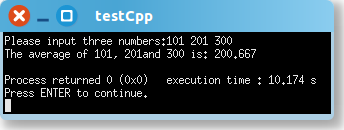
\includegraphics[width=0.45\textwidth]{chap02/01cppoutput01}
  \end{center}
\end{frame}  

\subsection[格式控制]{格式控制}
\begin{frame}[fragile]{输入输出}{输出格式设置}%
  \begin{itemize}
  \item 格式控制
  \end{itemize}
  \begin{spacing}{1.8}
  \begin{center}
    \scriptsize
    \begin{tabular}{|c|l|l|}
      \hline
      操作符 & 作用 & 说明 \\
      \hline
      \cppinttscr{oct} & 数据以8进制形式输出 & \multirow{3}{2cm}{作用范
                                              围为后续输出的整数,对小数不起作用}\\
      \cline{1-2}
      \cppinttscr{dec} & 数据以10进制形式输出(默认) & \\
      \cline{1-2}
      \cppinttscr{hex} & 数据以16进制形式输出 & \\
      \hline
      \cppinttscr{endl} & 换行并刷新输出流 & \\
      \hline
      \cppinttscr{setw(n)} & 设置输出宽度 & \multirow{2}{2cm}{作用范围为后续对象}\\
      \cline{1-2}
      \cppinttscr{setprecision(n)} & 设置输出精度(默认为6) & \\
      \hline
    \end{tabular}
    \begin{minipage}{0.65\linewidth}
      \scriptsize
      \begin{alertblock}{注意:}
        \begin{itemize}
        \item \cppinttscr{#include <iomanip>}
        \item 默认情况下, \cppinttscr{setprecision(n)}仅对带有小
          数的数有效, n为整数与小数位数之和
        \end{itemize}
      \end{alertblock}
    \end{minipage}
  \end{center}
  \end{spacing}
\end{frame}

\begin{frame}[fragile]{输入输出}{输出格式设置}%label=testframe,
  \begin{itemize}
  \item 设置输出格式
  \end{itemize}
  \begin{center}
    \begin{tikzpicture}[show background grid]
      \tiny
      \umlnote[scale=0.95, text width=0.55\textwidth](code1) at (0, 0)
      {
        \cppfiletikz{codes/chap02/ex02-02.cpp}
      };
    \end{tikzpicture}
    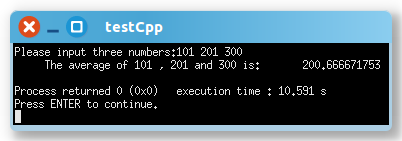
\includegraphics[width=0.45\textwidth]{chap02/01cppoutput02}
  \end{center}
\end{frame}  

  
%%%%%%%%%%%%%%%%%%%%%%%%%%%%%%%%%%%%%%%%%%%%%%%%%%%%%%%%%%%%%%%%%%%%%%%%%% 

\section[类型与表达式]{基本数据类型与表达式}\label{sec:chap02-sec03}
\subsection[基本类型]{基本类型}
\begin{frame}[t, fragile]{类型与表达式}{基本数据类型}
  \stretchon
  \begin{itemize}
  \item 基本数据类型
    \begin{itemize}
    \item \cppinttfts{int}, \cppinttfts{float}, \cppinttfts{double}, \cppinttfts{void}, \cppinttfts{char}
    \item 布尔型:\cppinttfts{bool} (\cppinttfts{true}$\Rightarrow$1, \cppinttfts{false}$\Rightarrow$0)
    \end{itemize}
  \item 变量与常量
    \begin{itemize}
    \item 变量的定义与赋初值
      \begin{itemize}
      \item \cppinttscr{int sum=100; double pi=3.1416; char c='a';}
      \item \cppinttscr{int sum(100); double pi(3.1416); char c('a');}
      \end{itemize}
    \item 符号常量与常变量
      \begin{itemize}
      \item \cppinttscr{#define PI 3.1416}
      \item \cppinttscr{const float PI=3.1416;}
      \item \cppinttscr{PI = 3.1415926535898;      // 错误!}
      \end{itemize}
    \end{itemize}
  \end{itemize}
  \stretchoff
\end{frame}

\subsection[新类型]{C++新类型}
\begin{frame}[fragile]{类型与表达式}{C++11中的新类型}
  \stretchon
  \begin{itemize}
  \item 常量表达式\\
  %\begin{center}
    \begin{minipage}{0.85\linewidth}
      \begin{cppcode}
const int size = 20;          // size是常量表达式
const int limits = size + 1;  // limits是常量表达式
int max = 80;                 // max不是常量表达式,80是字面值常量,
                              // 但max不是const, 不保证运行是不变。
const int lines = get_size(); // lines不是常量表达式
                              // lines是常量,但get_size()运行时才能确定
      \end{cppcode}
    \end{minipage}
  %\end{center}
  \item  \cppinline{constexpr}类型(验证是不是常量表达式)\\
     \begin{minipage}{0.85\linewidth}
      \begin{cppcode}
constexpr int size = 20;           // 20是常量表达式
constexpr int limits = size + 10;  // size + 10是常量表达式
constexpr int max = length();      // 取决于length()函数是不是常量函数
      \end{cppcode}
    \end{minipage}
  \item \cppinline{constexpr}与\cppinline{const}\\
    \begin{minipage}{0.85\linewidth}
      \begin{cppcode}
constexpr int a = length(); // 必须在编译时能计算出length()返回值
const int b = length();     // b的值可以在运行时获得,之后不再改变
      \end{cppcode}
    \end{minipage}
  \end{itemize}
  \stretchoff
\end{frame}

\begin{frame}[fragile]{类型与表达式}{C++11中的新类型}
  \stretchon
  \begin{itemize}
  \item \cppinline{auto}类型说明符\\
  %\begin{center}
    \begin{minipage}{0.95\linewidth}
      \begin{cppcode}
auto x = 5;               // 5是int类型,x则是int类型
auto size = sizeof(int);  // size是表示内存字节数的类型
auto name = "world";      // name是保存字符串的类型
cout << "hello " << name; // 可以使用name
auto a;                   // 错误!没有初始值无法确定类型
auto r = 1, pi = 3.14;    // 错误!类型混淆
     \end{cppcode}
    \end{minipage}
  %\end{center}
  \item  \cppinline{decltype}类型指示符,\alert{返回操作数类型}\\
     \begin{minipage}{0.95\linewidth}
      \begin{cppcode}
decltype(sizeof(int)) size; // sizeof(int)结果的类型
const int ci = 0;           // 是常量表达式
decltype(ci) x = 1;         // const int 类型
decltype(f()) y = sum;      // 函数f()的返回值类型
      \end{cppcode}
    \end{minipage}
  \end{itemize}
  \stretchoff
\end{frame}

\subsection[运算符与表达式]{运算符与表达式}
\begin{frame}[fragile]{类型与表达式}{运算符与表达式}
  \begin{spacing}{1.3}
  \begin{itemize}
  \item 运算符与表达式
    \begin{itemize}
    \item 算术运算符:\cppinttfts{+(|正号|), -(|负号|), *, /, %(|取余|)}
    \item 关系运算符:\cppinttfts{>, <, >=, <=, ==, !=}
    \item 逻辑运算符:\cppinttfts[escapeinside=//]{!, &&, ||}
    \item 位运算符: \cppinttfts[escapeinside=//]{~, <<, >>, &, ^(/异或/), /|/}
    \item 赋值运算符:\cppinttfts{=, *=, /=, %=, +=, -=, |$\cdots$|}
    \item 递增递减运算符:\cppinttfts{++, --}
    \end{itemize}
  \end{itemize}
  \centering  
  \begin{minipage}{0.3\linewidth}
    \scriptsize
    \begin{gather*}
      ax^{2}+bx+c=0 \\
      x_{1,2}=\frac{-b \pm \sqrt{b^{2}-4ac}}{2a}
    \end{gather*}
  \end{minipage}\\
  \begin{minipage}{0.6\linewidth}
    \begin{cppcode}
if(abs(b * b - 4 * a * c) > 1.0e - 10)
{
    x1 = (-b + sqrt(b * b - 4 * a * c)) / (2 * a);
    x2 = (-b - sqrt(b * b - 4 * a * c)) / (2 * a);
}
    \end{cppcode}
  \end{minipage}
  
  \end{spacing}
\end{frame}
%%%%%%%%%%%%%%%%%%%%%%%%%%%%%%%%%%%%%%%%%%%%%%%%%%%%%%%%%%%%%%%%%%%%%%%%%%

\section[控制结构]{控制结构}\label{sec:chap02-sec04}
%%%%%%%%%%%%%%%%%%%%%%%%%% 控制结构 %%%%%%%%%%%%%%%%%%%%%%%%%%%%%
\subsection[基本结构]{基本结构}
\begin{frame}[t, fragile]{控制结构}{基本结构}
  \stretchon
  \begin{itemize}
  \item 判断
    \begin{itemize}
    \item \cppinttfts{if ... else ...}
    \item \cppinttfts{if ... else if ... else ...}
    \item \cppinttfts{switch ... case ...}
    \end{itemize}
  \item 循环
    \begin{itemize}
    \item \cppinttfts{for(exp1;exp2;exp3){...}}
    \item \cppinttfts{while(exp){...}}
    \item \cppinttfts{do ... while(exp);}
    \end{itemize}
  \item 转移
    \begin{itemize}
    \item \cppinttfts{break}
    \item \cppinttfts{continue}
    \item \cppinttfts{goto}
    \end{itemize}
  \end{itemize}
  \stretchoff
\end{frame}

\subsection[范围for语句]{范围for语句}
\begin{frame}[fragile]{控制结构}{C++11中的范围for语句}
  \stretchon
  \begin{itemize}
  \item 范围\cppinline{for}语句\\[-1ex]
  %\begin{center}
    \begin{minipage}{0.95\linewidth}
      \begin{cppcode}
for(declaration : expression){
  statement;
}
// 其中:
//   expression必须是一个序列(列表、数组、vector、string等),
//     能返回begin和end对象。
//   declaration是一个变量,序列中每个元素都能够转换为该类型,
//     常用auto声明
      \end{cppcode}
    \end{minipage}
  %\end{center}
  \item 范围\cppinline{for}示例\\[-1ex]
     \begin{minipage}{0.95\linewidth}
      \begin{cppcode}
// 累加20以内的素数
int sum = 0;
for(int e : {2, 3, 5, 7, 11, 13, 17, 19}) // 用auto类型更合理
    sum += e;
cout << sum << endl;                      // 输出结果77
int arr[] = {1, 3, 5, 7, 9};              // 声明数组arr,初始化为5个奇数
for(auto ele : arr){                      // 声明ele,与数组arr关联在一起,用了auto
  ele = ele * 2;                          // 修改数组每个元素的值
  cout << ele << " ";                     // 输出ele,2 6 10 14 18
}
cout << endl;
for(auto ele : arr)
    cout << ele << " ";                   // 没有改变:1 3 5 7 9
cout << endl;
      \end{cppcode}
    \end{minipage}
  \end{itemize}
  \stretchoff
\end{frame}
%%%%%%%%%%%%%%%%%%%%%%%%%%%%%%%%%%%%%%%%%%%%%%%%%%%%%%%%%%%%%%%%%%%%%%%%%% 

\section[复杂类型]{复杂数据类型}\label{sec:chap02-sec05}
%%%%%%%%%%%%%%%%%%%%%%%%%%%%%%%% 构造数据类型 %%%%%%%%%%%%%%%%%%%%%%%%%%%%%%%%%%
% \begin{frame}[t, fragile]{复杂类型}{枚举和数组}
%   \stretchon
%   \begin{itemize}
%   \item 枚举类型
%     \begin{itemize}%\mintinline{c++}{}
%     \item \cppinline{enum weekday{SUN, MON,...,SAT};}
%     \end{itemize}
%   \item 数组
%     \begin{itemize}
%     \item 一维数组定义与初始化\\
%       \cppinline{int a[4]={1,2,3,4}; }\\
%       \cppinline{int a[]={1,2,3,4};}\\
%       \cppinline{char str[256]="movie.rm";}\\
%       \cppinline{char str[] = "movie.rm";}
%     \item 二维数组定义与初始化\\
%       \cppinline{int a[3][3]={{1,2,3},{4,5,6},{7,8,9}};}\\
%       \cppinline{int a[][3]={{1,2,3},{4,5,6},{7,8,9}};}
%     \end{itemize}  
%   \end{itemize}
%   \stretchoff
% \end{frame}
\subsection[指针与内存]{指针与内存}
\begin{frame}[t, fragile]{复杂类型}{指针}
  \begin{itemize}  
  \item 指针    
  \end{itemize}
  \hfill
  \begin{minipage}{0.35\linewidth}
    \begin{cppcode}    
int a=255;
int *p;
p=&a;
    \end{cppcode}
  \end{minipage}
  \begin{minipage}{0.6\linewidth}
    \tiny
    \begin{bytefield}{24}
      \begin{rightwordgroup}{\&a}
        \memsection[\&p$\rightarrow$]{0x00ff ffee}{0x00ff fffb}{4}{00FF 4212}
      \end{rightwordgroup}\\
      \memsection{}{}{4}{\ldots\ldots}\\
      \begin{rightwordgroup}{a}
        \memsection[\&a$\to$]{0x00ff 4212}{0x00ff 420f}{4}{0000 00FF}
      \end{rightwordgroup}\\
    \end{bytefield}
  \end{minipage}\\
  \begin{center}
    \begin{minipage}{0.7\linewidth}
      \begin{cppcode}      
float x[5];
float *p = x;
double sum = 0.0;
for (int i = 0; i < 5; i++)
{
  sum += *p++;
}      
      \end{cppcode}
    \end{minipage}
  \end{center}
\end{frame}

%\subsection[动态内存分配]{动态内存分配}
\begin{frame}[fragile]{复杂类型}{动态内存分配}
  \begin{itemize}
  \item 动态内存分配    
    \begin{itemize}
    \item \cppinttfts{malloc}和\cppinttfts{free}
    \item \cppinttfts{new}和\cppinttfts{delete}
    \end{itemize}  
  \end{itemize}
  \begin{center}
    \begin{minipage}{0.55\linewidth}
      \begin{cppcode}
// C语言
float *x = (float *)malloc(n*sizeof(float));
free (x);

// C++语言
float *x = new float[n];
delete []x;
      \end{cppcode}
    \end{minipage}\\%qquad
    \begin{minipage}{0.35\linewidth}
      \begin{cppcode}
int **mat;
int m, n;
mat = new int *[m];

for (i = 0; i < m; i++)
    mat[i] = new int[n];

for (i = 0; i < m; i++)
    delete [] mat[i];
delete [] mat;
      \end{cppcode}
    \end{minipage}
  \end{center}
\end{frame}
%\subsection[定位new表达式]{定位new表达式}
\begin{frame}[fragile]{复杂类型}{动态内存分配}
  \begin{itemize}
  \item 定位\cppinline{new}表达式
    \begin{itemize}
    \item 语法:\cppinttfts{new (|指针|)|类型|}
    \end{itemize}  
  \end{itemize}
  \begin{center}
    \begin{minipage}{0.7\linewidth}
      \begin{cppcode}
#include <iostream>
#include <new> // 必须包含该头文件

using namespace std;

char * buf = new char[1000]; // 预分配空间        

int main()
{
    int * pi = new (buf) int; // 在buf中创建一个int对象

    return 0;
}
      \end{cppcode}
    \end{minipage}
  \end{center}
\end{frame}

\subsection[指针与常量]{指针与常量}
\begin{frame}[t,fragile]{复杂类型}{指针常量和常量指针}
  \begin{itemize}
  \item 指针常量\\
    \begin{center}
      \begin{minipage}{0.6\linewidth}
        \begin{cppcode}
int a = 2, b = 3;
int * const p = &a;  //定义时必须赋初值
p = &b;              //错误,地址不能被修改
*p = b;              //正确,内容可以被修改
        \end{cppcode}
      \end{minipage}
    \end{center}
  \item 常量指针\\
    \begin{center}
      \begin{minipage}{0.55\linewidth}
        \begin{cppcode}
int a = 2, b = 3;
const int * p; 
p = &b;         //正确,地址可以被修改
*p = b;         //错误,内容不可以被修改
        \end{cppcode}
      \end{minipage}
    \end{center}
  \item 常指针常量\\
    \begin{center}
      \begin{minipage}{0.65\linewidth}
        \begin{cppcode}
int a = 2, b = 3;
const int * const p = &a;  //定义时必须赋初值
p = &b;         //错误,地址不能被修改
*p = b;         //错误,内容不可以被修改
        \end{cppcode}
      \end{minipage}
    \end{center}
  \end{itemize}
\end{frame}
\subsection[引用类型]{引用类型}
\begin{frame}[t, fragile]{复杂类型}{引用类型}
  \begin{itemize}
  \item 引用是已存在的变量的别名\\
    \begin{center}
      \begin{minipage}{0.6\linewidth}
        \begin{cppcode}
int i = 3;
int &j = i;   //引用必须赋初值
int &j = 3;   //错误,初值必须为变量
j = 4;
        \end{cppcode}
      \end{minipage}
    \end{center}
  \item 引用和指针的区别与联系\\
    \begin{center}
      \begin{minipage}{0.45\linewidth}
        \begin{cppcode}
int i = 3;
int &j = i;
int *k = &i;
cout << &i << endl;
cout << &j << endl;
cout << &k << endl;
        \end{cppcode}
      \end{minipage}
      \begin{minipage}{0.5\linewidth}
        \tiny
        \begin{bytefield}{24}
          \memsection{$\cdots$}{}{1}{$\cdots$}\\
          \memsection[k$\rightarrow$]{0x0016 FDEC}{}{1}{0x0016 FE04}\\
          \memsection{$\cdots$}{}{1}{$\cdots$}\\
          \memsection[$\genfrac{}{}{0pt}{}{\texttt{i}}{\texttt{j}}\rightarrow$]{0x0016 FE04}{}{1}{0x0000 0003}\\
          \memsection{$\cdots$}{}{1}{$\cdots$}
        \end{bytefield}
      \end{minipage}
    \end{center}
  \end{itemize}
\end{frame}

\begin{frame}[t, fragile]{复杂类型}{引用类型}
  \begin{itemize}
  \item 引用作为函数参数(例1)\\[-0.5ex]
    \begin{center}
      \scalebox{0.8}{
        \begin{minipage}{0.5\linewidth}
          \cppfile[fontsize=\scriptsize]{codes/chap02/ex02-03.cpp}
        \end{minipage}\qquad\qquad
        \begin{minipage}{0.5\linewidth}
          \cppfile[fontsize=\scriptsize]{codes/chap02/ex02-04.cpp}
        \end{minipage}
      }
    \end{center}
  \end{itemize}
\end{frame}

% \begin{frame}[t, label=testframe, fragile]{输出格式设置}%label=testframe,
%   \begin{center}
%     \begin{tikzpicture}[show background grid]
%       \tiny
%       \umlnote[text width=0.75\textwidth](code1) at (0, 0)
%       {
%         \cppfiletikz{codes/chap02/ex02-02.cpp}
%       };
%     \end{tikzpicture}
%     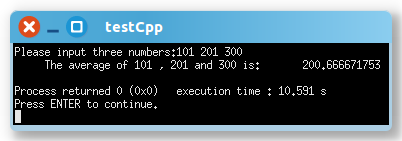
\includegraphics[width=0.5\textwidth]{chap02/01cppoutput02}
%   \end{center}
% \end{frame} 


\begin{frame}[t, fragile]{复杂类型}{引用类型}
  \begin{itemize}
  \item 引用作为函数参数(例2)\\
    \begin{center}
      \begin{minipage}{0.35\linewidth}
        \begin{cppcode}
struct StuNode
{
    int ID;
    char name[128];
    bool gender;
    int age;
    struct StuNode *next;
};
        \end{cppcode}
      \end{minipage}\qquad
      \begin{minipage}{0.5\linewidth}
        \begin{tikzpicture}[show background grid]
          \tiny
          \umlnote[text width = 0.85\textwidth](code1) at (0, 0)
          {
            \cppfiletikz{codes/chap02/ex02-05.cpp}
          };          
        \end{tikzpicture}        
        %\cppfile{codes/chap02/ex02-05.cpp}
      \end{minipage}
    \end{center}
  \end{itemize}
\end{frame}

\begin{frame}[t, fragile]{复杂类型}{引用类型}
  \begin{itemize}
  \item 引用作为函数参数(例2)\\
    \begin{center}
      \begin{minipage}{0.35\linewidth}
        \begin{cppcode}
struct StuNode
{
  int ID;
  char name[128];
  bool gender;
  int age;
  struct StuNode *next;
};
        \end{cppcode}
      \end{minipage}\qquad
      \begin{minipage}{0.5\linewidth}
        \begin{tikzpicture}[show background grid]
          \tiny
          \umlnote[text width = 0.85\textwidth](code1) at (0, 0)
          {
            \cppfiletikz{codes/chap02/ex02-06.cpp}
          };          
        \end{tikzpicture}
        %\cppfile{codes/chap02/ex02-06.cpp}
      \end{minipage}
    \end{center}
  \end{itemize}
\end{frame}

\begin{frame}[t,fragile]{复杂类型}{引用类型}
  \begin{itemize}
  \item 常引用\\
    \begin{minipage}{0.8\linewidth}
      \begin{cppcode}
int i = 100;
const int &r1 = 100;            //正确
const int &r2 = i;              //必须初始化
r2 = 200;                       //错误
      \end{cppcode}
    \end{minipage}
  \item 常引用参数\\
    \begin{minipage}{0.8\linewidth}
      \begin{cppcode}
int fun(const int &a, const int &b)
{
    return (a + b) / 2;         //参数不能被修改
}
      \end{cppcode}
    \end{minipage}
  \end{itemize}
\end{frame}

\begin{frame}[t,fragile]{复杂类型}{引用类型}
  \begin{itemize}
  \item 常引用\\
    \begin{minipage}{0.8\linewidth}
      \begin{cppcode}
int i = 100;
const int &r1 = 100;            //正确
const int &r2 = i;              //必须初始化
r2 = 200;                       //错误
      \end{cppcode}
    \end{minipage}
  \item 常引用参数\\
    \begin{minipage}{0.8\linewidth}
      \begin{cppcode}
int fun(const int &a, const int &b)
{
    return (a + b) / 2;         //参数不能被修改
}
      \end{cppcode}
    \end{minipage}
  \end{itemize}
\end{frame}
\subsection[C++类类型]{C++类类型}
\begin{frame}[fragile]{复杂类型}{迭代器}
  \begin{itemize}
  \item \cppinline{begin()}和\cppinline{end()}
    \begin{itemize}
    \item 语法\\
      \begin{center}
        \begin{minipage}{0.6\linewidth}
          \begin{cpptt}
begin(|\emph{数组名}|)
end(|\emph{数组名}|)
          \end{cpptt}
          \end{minipage}
      \end{center}
    \end{itemize}
  \item 运算
    \begin{itemize}
    \item 解引用
    \item 自增、自减
    \item 加或减整数、
    \item 指针相减
    \item 指针比较
    \end{itemize}
  \end{itemize}
  \begin{center}
    \begin{minipage}{0.6\linewidth}
      \begin{cppcode}
#include<iterator>  // 迭代器运算头文件
...
int ia[5] = {1, 2, 3, 4, 5};
int *pb = begin(ia);
int *pe = begin(ia);
while(pb != pe && *pb >= 0)
{
  ++pb;
}
      \end{cppcode}
    \end{minipage}
  \end{center}
\end{frame}
%\subsection[字符串]{字符串}
\begin{frame}[fragile]{复杂类型}{字符串}
  \stretchon
  \begin{itemize}
  \item 字符数组和C风格字符串
    \begin{itemize}
    \item 以\cppinttfts{'\0'}结束字符串
    \item 需要使用头文件:\cppinttfts{#include<cstring>}
    \end{itemize}
  \item C++的\cppinttfts{string}类
    \begin{itemize}
    \item 需要使用头文件:\cppinttfts{#include<string>}
    \item 丰富的字符串处理函数
    \item 便捷的运算符重载
    \item 单字符处理
      \begin{itemize}
      \item 需要使用头文件:\cppinttfts{#include<cctype>}
      \item 基本循环
      \item 范围for
      \end{itemize}
    \end{itemize}
  \end{itemize}
  \stretchoff
\end{frame}
%\subsection[vector向量]{vector向量}
\begin{frame}[fragile]{复杂类型}{向量}
  \stretchon
  \begin{itemize}
  \item 标准类型\cppinline{vector}
    \begin{itemize}
    \item 同种类型对象的集合
    \item 长度可变
    \end{itemize}
  \item 定义和初始化
    \begin{itemize}
    \item 语法:\cppinttfts{vector<|\emph{元素类型}|> |\emph{变量名}|;}
    \item 初始化方法\\[2ex]
      \tiny
      \begin{tabular}{l|l}
        %\scriptsize
        \toprule
        \multicolumn{1}{c|}{\emph{方 \qquad 法}} & \multicolumn{1}{c}{\emph{说 \qquad 明}} \\ \midrule
        \cppinttscr{vector<T> v1} & v1为空,元素是T类型,默认初始化 \\ \midrule
        \cppinttscr{vector<T> v2(v1)} & 声明v2向量,用v1初始化,是v1的副本 \\ \midrule
        \cppinttscr{vector<T> v2 = v1} & 等价于v2(v1) \\ \midrule
        \cppinttscr{vector<T> v3(n, val)} & v3有n个T类型的\alert{重复}元素,每个元素的值都是val\\ \midrule
        \cppinttscr{vector<T> v4(n)} & v4有n个\alert{重复}默认值初始化的元素 \\ \midrule
        \cppinttscr{vector<T> v5{a,b,c,...}} & v5元素个数为初始化式中元素个数 \\ \midrule
        \cppinttscr{vector<T> v5={a,b,c,...}} & 等价于v5\{a,b,c,...\} \\ \bottomrule
      \end{tabular}
    \end{itemize}
  \end{itemize}
  \stretchoff
\end{frame}
\subsection[类型转换]{类型转换}
\begin{frame}[fragile]{复杂类型}{类型转换}
  \stretchon
  \begin{itemize}
  \item 强制类型转换
    \begin{itemize}
    \item C风格\\
      \begin{cppcode}
float x = 3.5;
int roundX = (int)(x + 0.5);
      \end{cppcode}
    \item C++风格:\cppinttfts{castname<|\emph{类型名}|>(|\emph{表达式}|)}\\      
      \begin{itemize}
      \item \cppinttscr{static_cast}
      \item \cppinttscr{dynamic_cast}
      \item \cppinttscr{const_cast}
      \item \cppinttscr{reinterpret_cast}
      \end{itemize}
      \begin{cppcode}
int roundX = static_cast <int> (x+0.5);
      \end{cppcode}
    \end{itemize}
  \item 强制指针类型转换\\
    \begin{cppcode}
char *p;
void *q = malloc(sizeof(char)*1024);
p = q;    //错误!无法从“void *”转换为“char *”,C++
p =  (char *)q; 
    \end{cppcode}
  \end{itemize}
  \stretchoff
\end{frame}
%%%%%%%%%%%%%%%%%%%%%%%%%%%%%%%%%%%%%%%%%%%%%%%%%%%%%%%%%%%%%%%%%%%%%%%%%%

\section[函数]{函数}\label{sec:chap02-sec06}
%%%%%%%%%%%%%%%%%%%%%%%%%%%%%%%% 基本C++程序 %%%%%%%%%%%%%%%%%%%%%%%%%%%%%%%%%%
\begin{frame}{函数}{概述}
  \stretchon
  \begin{itemize}
  \item 函数调用执行过程
  \item 内联函数
  \item 带默认形参的函数
  \item 函数重载
  \item 函数模板
  \item 系统函数
  \end{itemize}
  \stretchoff
\end{frame}

\begin{frame}[fragile]{函数}{函数调用执行过程}
  \begin{itemize}
  \item 函数调用
    \begin{itemize}
    \item 参数和函数返回地址入栈
    \end{itemize}
  \item 执行函数体
    \begin{itemize}
    \item 寄存器进出栈,通过栈访问参数
    \end{itemize}
  \item 函数返回
    \begin{itemize}
    \item 返回到调用函数的下一条语句执行
    \end{itemize}
  \end{itemize}
  \begin{center}
    \begin{minipage}{0.3\linewidth}
      \begin{cppcode}
int increase(int a)
{
  return ++a;
}
int main()
{
  int x =3,y;
  y = increase(x);
  return 0;
}
      \end{cppcode}
    \end{minipage}
    \begin{minipage}{0.6\linewidth}
      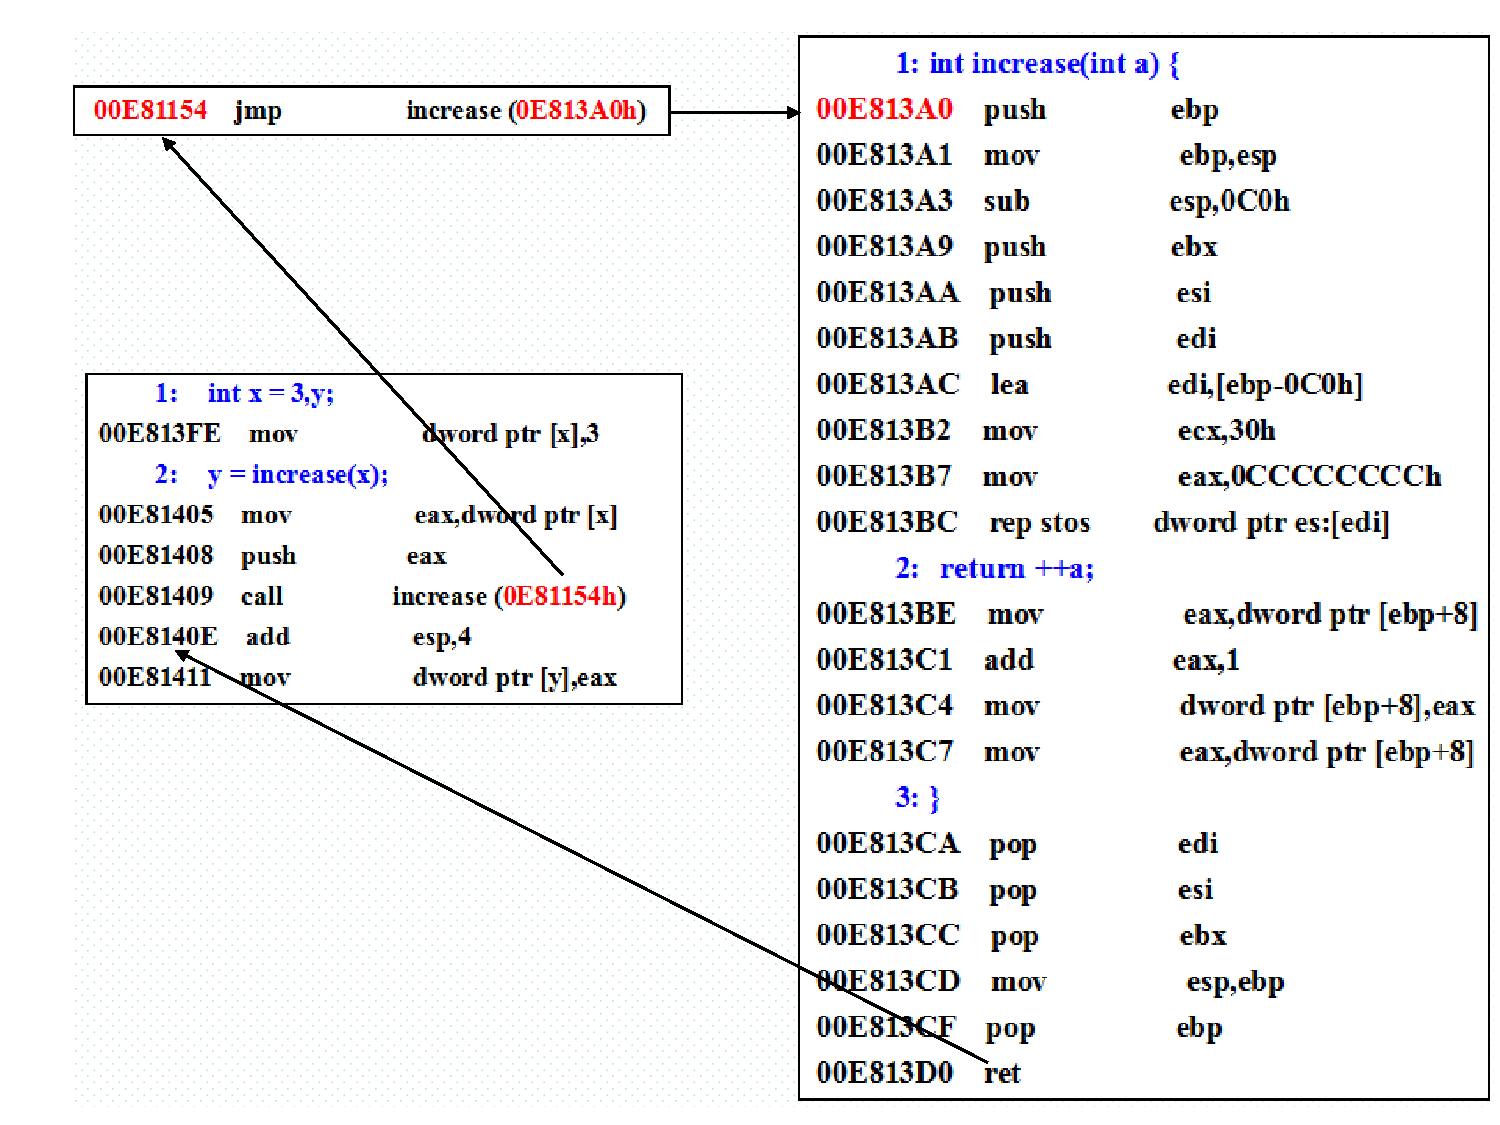
\includegraphics[width=0.8\textwidth]{chap02/03funasm}
    \end{minipage}
  \end{center}
\end{frame}
\subsection[内联函数]{内联函数}
\begin{frame}[fragile]{函数}{内联函数}
  \stretchon
  \begin{itemize}
  \item 普通函数调用缺陷
    \begin{itemize}
    \item 时间开销
    \end{itemize}
  \item 内联函数
    \begin{itemize}
    \item 在编译时将函数体代码插入到调用处
    \item 适用于代码短、频繁调用的场合
    \end{itemize}
  \item 定义\\[2ex]
    %\begin{center}
      \begin{minipage}{0.6\linewidth}
        \begin{cpptt}
inline |函数类型| |函数名|(|参数表|)
{
    |函数体|;
}
       \end{cpptt}
      \end{minipage}
    %\end{center}
  \end{itemize}
  \stretchoff
\end{frame}

\begin{frame}[fragile]{函数}{内联函数}
  \begin{itemize}
  \item 本质是预处理后展开\\
    \begin{center}
      \begin{minipage}{0.4\linewidth}
        \begin{cppcode}
inline int increase(int a)
{
  return ++a;
}
int main()
{
  int x = 3,y;
  y = increase(x);
  return 0;
}
        \end{cppcode}
      \end{minipage}$\Longrightarrow$
      \begin{minipage}{0.3\linewidth}
        \begin{cppcode}
int main()
{
  int x = 3,y;
  int a = x;
  y = ++a;
  return 0;
}
        \end{cppcode}
      \end{minipage}
    \end{center}
  \item 效率测试\\
    \begin{center}
      \begin{minipage}{0.56\linewidth}
        \begin{cppcode}
inline float getCos_inline(int &x)
{
  float r;
  x = rand();
  r = cos(2 * 3.1416 * x / (float)RAND_MAX);
  return r;
}
        \end{cppcode}
      \end{minipage}
      \begin{minipage}{0.4\linewidth}
        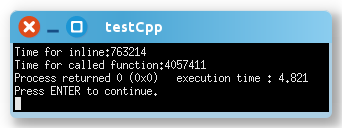
\includegraphics[width=0.8\textwidth]{chap02/04inlinetest}\\
        \tiny
        测试环境 (Code:Blocks GCC Release)\\
        效率比 = 4057411ms/763214ms = 5.3
        \colorbox{yellow}{\textcolor{blue}{例02-07:ex02-07.cpp}}
      \end{minipage}
    \end{center}
  \end{itemize}
\end{frame}

\begin{frame}[fragile]{函数}{内联函数}
  \stretchon
  \begin{itemize}
  \item 注意事项
    \begin{itemize}
    \item 不能出现递归
    \item 代码不宜过长
    \item 不宜出现循环
    \item 不宜含有复杂控制语句如\cppinttfts{switch}等
    \item 有些编译器会智能处理是否为内联函数
    \end{itemize}
  \end{itemize}
  \stretchoff
\end{frame}
\subsection[constexpr函数]{constexpr函数}
\begin{frame}[fragile]{函数}{constexpr函数}
  \stretchon
  \begin{itemize}
  \item 语法
    \begin{itemize}
    \item \cppinttfts{constexpr |\emph{函数}|(|\emph{常量表达式函数}|)}
    \end{itemize}
  \item 基本要求
    \begin{itemize}
    \item 只有一句\cppinttfts{return}可执行语句,可有别名、
      \cppinttfts{using}等
    \item 必须有返回类型,返回类型不能是\cppinttfts{void}
    \item 使用前必须定义(不只是声明)
    \item \cppinttfts{return}中不能有非常量表达式
    \end{itemize}
  \end{itemize}
  \stretchoff
\end{frame}

\begin{frame}[fragile]{函数}{constexpr函数}
  \stretchon
  \begin{itemize}
  \item 是编译时求值,不是运行是调用\\[-1.5ex]
    \begin{cppcode}
constexpr int data() // 错误,函数体只能有一条return可执行语句
{
  const int i = 1;
  return i;
}
constexpr int data() // 正确
{
  return 1;
}
constexpr void f()   // 错误,无法获得常量
{
}
    \end{cppcode}
  \item 是函数使用(\alert{编译时}),不是函数调用(\alert{运行时})\\[-1.5ex]
    \begin{cppcode}
constexpr int f();     // 只有constexpr函数的声明,没有定义
int a = f();           // 正确,可以将编译时的计算转换为运行时的调用
const int b = f();     // 正确,编译器将f()转换为一个运行时的调用
constexpr int c = f(); // 错误,c是constexpr,要求使用f(),在编译时计算
constexpr int f()      // constexpr函数的定义
{
  return 1;
}
constexpr int d = f(); // 正确,f()已定义,可以使用f()
    \end{cppcode}
  \end{itemize}
  \stretchoff
\end{frame}

\begin{frame}[fragile]{函数}{constexpr函数}
  \stretchon
  \begin{itemize}
  \item \cppinline{return}中不能包含运行时才能确定的函数\\[-1.5ex]
    \begin{cppcode}
const int e() 
{        
  return 1;
}
constexpr int g()
{
  return e();     // 错误,调用了非constexpr函数
}
constexpr int e() 
{        
  return 1;
}
constexpr int g() 
{
  return e();     // 正确,函数e()是常量表达式函数
}
    \end{cppcode}
  \item 用\cppinline{constexpr}函数初始化\cppinline{constexpr}变量\\[-1.5ex]
    \begin{cppcode}
constexpr int new_sz()
{
  return 100;
}
constexpr int size = new_sz();
    \end{cppcode}
  \end{itemize}
  \stretchoff
\end{frame}
\subsection[形参默认值]{形参默认值}
\begin{frame}[fragile]{函数}{带默认形参值的函数}
  \begin{spacing}{1.8}
    \begin{itemize}
    \item 在函数定义或说明中\alert{为形参赋默认值}
    \item 作用
      \begin{itemize}
      \item 若调用给出实参值,则形参采用实参值
      \item 若调用未给出实参值,则调用默认参数值
      \end{itemize}
    \end{itemize}
  \end{spacing}
  \vspace{-2ex}
  \begin{center}
    \begin{minipage}{0.9\linewidth}
      \cppfile{codes/chap02/ex02-08.cpp}
    \end{minipage}
  \end{center}
\end{frame}

\begin{frame}[fragile]{函数}{带默认形参值的函数}
  \begin{spacing}{1.8}
    \begin{itemize}
    \item \alert{基本要求}
      \begin{itemize}
        \scriptsize
      \item 调用函数时,如省去某个实参,则该实参右边所有实参都要省略
      \item 默认形参必须\alert{自最右向左连续}定义
      \item 若函数声明(原型)中给出默认形参值,则函数定义时不能重复指定
      \end{itemize}
    \end{itemize}
  \end{spacing}
  \vspace{-3ex}
  \begin{center}
    \begin{minipage}{0.9\linewidth}
      \cppfile{codes/chap02/ex02-09.cpp}
    \end{minipage}
  \end{center}
\end{frame}

\begin{frame}[fragile]{函数}{带默认形参值的函数}
  \begin{itemize}
  \item \alert{中间参数不能省略}
  \end{itemize}
  \begin{center}
    \begin{minipage}{0.9\linewidth}
      \begin{tikzpicture}[show background grid]
        %\tiny
        \umlnote[text width = 1.00\textwidth](code1) at (0, 0)
        {
          \cppfiletikz{codes/chap02/ex02-10.cpp}
        };
      \end{tikzpicture}
      %\cppfile{codes/chap02/ex02-10.cpp}
    \end{minipage}
  \end{center}
\end{frame}

\begin{frame}[fragile]{函数}{带默认形参值的函数}
  \begin{itemize}
  \item \alert{不可重复指定参数默认值}
  \end{itemize}
  \begin{center}
    \begin{minipage}{0.9\linewidth}
      \cppfile{codes/chap02/ex02-11.cpp}
    \end{minipage}
  \end{center}
\end{frame}

\begin{frame}[fragile]{函数}{带默认形参值的函数}
  \begin{itemize}
  \item 默认形参必须\alert{自最右向左连续}定义
  \end{itemize}
  \begin{center}
    \begin{minipage}{0.9\linewidth}
      \cppfile{codes/chap02/ex02-12.cpp}
    \end{minipage}
  \end{center}
\end{frame}

\begin{frame}[fragile]{函数}{带默认形参值的函数}
  \begin{itemize}
  \item 默认形参必须\alert{自最右向左连续}定义
  \end{itemize}
  \begin{center}
    \begin{minipage}{0.9\linewidth}
      \cppfile{codes/chap02/ex02-13.cpp}
    \end{minipage}
  \end{center}
\end{frame}

\begin{frame}[fragile]{函数}{带默认形参值的函数}
  \begin{itemize}
  \item 必须为无默认值的参数提供实参
  \end{itemize}
  \begin{center}
    \begin{minipage}{0.9\linewidth}
      \begin{tikzpicture}[show background grid]
        %\tiny
        \umlnote[text width = 1.0\textwidth](code1) at (0, 0)
        {
          \cppfiletikz{codes/chap02/ex02-14.cpp}
        };
      \end{tikzpicture}
      %\cppfile{codes/chap02/ex02-14.cpp}
    \end{minipage}
  \end{center}
\end{frame}

\begin{frame}[fragile]{函数}{带默认形参值的函数}
  \begin{itemize}
  \item 形参的初始化可以是函数
  \end{itemize}
  \begin{center}
    \begin{minipage}{0.9\linewidth}
      \cppfile{codes/chap02/ex02-15.cpp}
    \end{minipage}
  \end{center}
\end{frame}
\subsection[重载函数]{重载函数}
\begin{frame}[fragile]{函数}{函数重载}
  \stretchon
  \begin{itemize}
  \item 重载:同一符号或函数名对应多种操作
    \begin{itemize}
    \item 操作符重载
    \item 函数重载
    \end{itemize}
  \item 函数重载
    \begin{itemize}
    \item 共性函数拥有相同函数名字\\
      \begin{cppcode}
int sum_int(int *a, int size);
float sum_float(float *a, int size);
double sum_double(double *a, int size);
      \end{cppcode}
      \vspace{-2ex}
      \begin{cppcode}
int sum(int *a, int size);
float sum(float *a, int size);
double sum(double *a, int size);
      \end{cppcode}
    \end{itemize}
  \end{itemize}
  \stretchoff
\end{frame}

\begin{frame}[fragile]{函数}{函数重载}
  \stretchon
  \begin{itemize}
  \item C++函数重载实现机理
    \begin{itemize}
    \item 函数名
    \item 参数类型
    \item 参数个数
    \end{itemize}
  \item 参数个数不同情况下的实现重载
    \begin{itemize}
      \begin{cppcode}
float dis_2d(float x0, float y0, float x1, float y1);
float dis_3d(float x0, float y0, float z0,
             float x1, float y1, float z1);
      \end{cppcode}
      \vspace{-2ex}
      \begin{cppcode}
float dis(float x0, float y0, float x1, float y1);
float dis(float x0, float y0, float z0,
          float x1, float y1, float z1);
      \end{cppcode}
    \end{itemize}
  \end{itemize}
  \stretchoff
\end{frame}

\begin{frame}[fragile]{函数}{函数重载}
  \stretchon
  \begin{itemize}
  \item 注意事项
    \begin{itemize}
    \item 避免二义性\\
      %\begin{center}
        \begin{minipage}{0.5\linewidth}
          \begin{cppcode}
void my_fun(int a, int b);
void my_fun(int &a, int &b);
          \end{cppcode}
        \end{minipage}
      %\end{center}
    \item 避免将不适宜重载的函数重载\\
      {\tiny 如果不同的函数名所提供的信息可使程序更容易理解,则不必使用重载}
      %\begin{center}
        \begin{minipage}{0.5\linewidth}
          \begin{cppcode}
void rotate(float r);
void translate(float x, float y);
          \end{cppcode}
          \vspace{-2ex}
          \begin{cppcode}
void transform(float r);
void transform(float x, float y);
          \end{cppcode}
        \end{minipage}
      %\end{center}
    \end{itemize}
  \end{itemize}
  \stretchoff
\end{frame}
\subsection{函数模板}
\begin{frame}[fragile]{函数}{函数模板}
  \stretchon
  \begin{itemize}
  \item 用一个函数表示逻辑功能相同但参数类型不同的函数\\
    %\begin{center}
      \begin{minipage}{0.6\linewidth}
        \begin{cppcode}
int sum(int *a, int size);
float sum(float *a, int size);
double sum(double *a, int size);
        \end{cppcode}
      \end{minipage}
    %\end{center}
  \item 定义\\
    %\begin{center}
      \tiny
      \begin{minipage}{0.8\linewidth}
        \mintinline{cpp}{template <class} 类型名1,
        \mintinline{cpp}{class} 类型名1, \ldots \mintinline{cpp}{>}
        返回类型~函数名(形参表)\\
        \{\\
            函数体;\\
        \}
      \end{minipage}\\
      \begin{minipage}{0.6\linewidth}
        \cppfile{codes/chap02/ex02-16.cpp}
      \end{minipage}
    %\end{center}
    \end{itemize}
  \stretchoff  
\end{frame}

\begin{frame}[fragile]{函数}{函数模板}
  \begin{itemize}  
  \item 带有两个通用类型的函数模板\\
    \begin{center}      
      \begin{minipage}{0.6\linewidth}
        \cppfile{codes/chap02/ex02-17.cpp}
      \end{minipage}
    \end{center}
  \end{itemize}
\end{frame}

\begin{frame}[fragile]{函数}{函数模板}
  \stretchon
  \begin{itemize}  
  \item 优先级别
    \begin{itemize}
    \item 如果同时定义重载函数,将优先使用重载函数,若不能找到精确匹配,再使用函数模板
    \end{itemize}
  \item 应用
    \begin{itemize}
    \item 数据结构中的链表、堆栈等
    \item C++的标准模板库(排序等)
    \item 通用类
    \end{itemize}
  \end{itemize}
  \stretchoff
\end{frame}

\begin{frame}[fragile]{函数}{函数模板}
  \begin{itemize}  
  \item 应用(例:冒泡排序)\\
    \begin{center}      
      \begin{minipage}{0.6\linewidth}
        \cppfile{codes/chap02/ex02-18.cpp}
      \end{minipage}
    \end{center}
  \end{itemize}
\end{frame}
\subsection{系统函数}
\begin{frame}[fragile]{函数}{系统函数}
  \stretchon
  \begin{itemize}  
  \item cmath
  \item iostream
    \begin{itemize}
    \item 包含\cppinttfts{ctype.h, string.h, memory.h, stdlib.h}等
        \cppinttfts{isdigit(), strcpy(), memcpy(), atoi(), rand()}等
    \end{itemize}
  \item ctime
    \begin{itemize}
    \item \cppinttfts{time_t, clock()}等
    \end{itemize}
  \end{itemize}
  \stretchoff
\end{frame}  
%%%%%%%%%%%%%%%%%%%%%%%%%%%%%%%%%%%%%%%%%%%%%%%%%%%%%%%%%%%%%%%%%%%%%%%%%%


\section[程序结构]{大型程序结构控制}\label{sec:chap02-sec07}
%%%%%%%%%%%%%%%%%%%%%%%%%%%%%%%% 基本C++程序 %%%%%%%%%%%%%%%%%%%%%%%%%%%%%%%%%%
\begin{frame}[fragile]{程序结构}{extern和static}
  \begin{itemize}  
  \item \cppinline{extern}    
    \begin{itemize}
      \tiny
    \item 大型程序设计中所有模块共同使用的全局变量(函数)
    \item 在一个模块中定义全局变量(函数),其它模块中
      用\cppinttscr{extern}说明``外来''的全局变量(函数)
    \end{itemize}
  \end{itemize}
  \vspace{-4.5ex}
  \begin{columns}
    \centering
    \begin{column}{0.42\textwidth}
      \centering
      \cppfile{codes/chap02/ex02-19-01.cpp}%}
      \vspace{-6ex}
      \cppfile{codes/chap02/ex02-19-02.cpp}%}
    \end{column}
    \begin{column}{0.42\textwidth}
      \centering
      \cppfile{codes/chap02/ex02-19-00.cpp}\\[-0.5ex]%}
      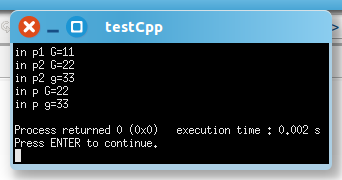
\includegraphics[width=0.8\textwidth]{chap02/05externkeyword}
    \end{column}
  \end{columns}
\end{frame}

\begin{frame}[fragile]{程序结构}{extern和static}
  \begin{itemize}  
  \item \cppinline{static}    
    \begin{itemize}
      \tiny
    \item \cppintttny{static}可用来声明全局静态变量和局部静态变量。当声明全局静态变
      量时,全局静态变量只能供本模块使用,不能被其它模块再声明
      为\cppintttny{extern}变量
    \end{itemize}
  \end{itemize}
  \begin{center}
    \begin{minipage}{0.4\linewidth}
      \cppfile{codes/chap02/ex02-20-01.cpp}
    \end{minipage}\qquad
    \begin{minipage}{0.4\linewidth}
      \cppfile{codes/chap02/ex02-20-02.cpp}
    \end{minipage}
  \end{center}
\end{frame}

\begin{frame}[fragile]{程序结构}{extern和static}
  \begin{itemize}  
  \item \cppinline{static}    
    \begin{itemize}
      \tiny
    \item 当一个局部变量声明为\cppintttny{static}变量,它既具有局部变量的性质,又具
      有全局变量的性质
    \end{itemize}
  \end{itemize}
  \begin{center}
    \begin{minipage}{0.53\linewidth}
      \cppfile{codes/chap02/ex02-21.cpp}
    \end{minipage}\qquad
    \begin{minipage}{0.35\linewidth}
      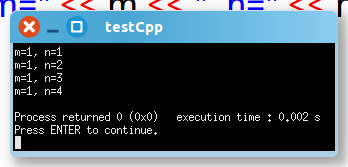
\includegraphics[width=0.8\textwidth]{chap02/06statickeyword}
    \end{minipage}
  \end{center}
\end{frame}

\begin{frame}[fragile]{程序结构}{包含头文件}
  \stretchon
  \begin{itemize}  
  \item 多文件操作使用\cppinline{#include}
  \item \cppintt{#include <|系统文件|>}
    \begin{itemize}
    \item 到编译器指定的文件包含目录查找
    \end{itemize}
  \item \cppintt{#include "|自定义文件.h"}
  \end{itemize}
  \stretchoff
\end{frame}

\begin{frame}[fragile]{程序结构}{条件编译}
  \begin{itemize}
  \item 同一程序在不同的编译条件下得到不同的目标代码
  \end{itemize}
  \begin{center}
    \begin{minipage}{0.6\linewidth}
      \cppfile{codes/chap02/ex02-22.cpp}
    \end{minipage}
  \end{center}
\end{frame}

\begin{frame}[fragile]{程序结构}{条件编译}
  \begin{itemize}
  \item 便于程序移植或跨平台
  \end{itemize}
  \begin{center}
    \begin{minipage}{0.4\linewidth}
      \cppfile{codes/chap02/ex02-23-01.cpp}
    \end{minipage}\qquad
    \begin{minipage}{0.4\linewidth}
      \cppfile{codes/chap02/ex02-23-02.cpp}
    \end{minipage}
  \end{center}
\end{frame}

\begin{frame}[fragile]{程序结构}{条件编译}
  \begin{itemize}
  \item 避免重复包含头文件如``MyHeader.h''\\
    \begin{center}
      \begin{minipage}{0.4\linewidth}
        \cppfile{codes/chap02/ex02-24.cpp}
      \end{minipage}
    \end{center}
  \item 便于调试程序\\
    \begin{center}
      \begin{minipage}{0.4\linewidth}
        \cppfile{codes/chap02/ex02-25.cpp}
      \end{minipage}
    \end{center}
  \end{itemize}
\end{frame}

\begin{frame}[fragile]{程序结构}{名字空间}
  \stretchon
  \begin{itemize}
  \item 不同程序员撰写的软件模块可能使用相同标志符
  \item 为避免冲突,将可能存在相同标志符的程序模块放入名字空间
  \item 定义:\\
    %\begin{center}
    \begin{minipage}{0.8\linewidth}
      \begin{cpptt}
namespace |名称|
{
   |成员变量或成员函数|;
}
        \end{cpptt}
      \end{minipage}
    %\end{center}    
    \end{itemize}
    \stretchoff
\end{frame}

\begin{frame}[fragile]{程序结构}{名字空间}
  \begin{itemize}
  \item 声明方式(作用域分辨符)\\
    名字空间名\cppinline{::}成员变量或成员函数\\
    \begin{center}
      \begin{minipage}{0.45\linewidth}
        \cppfile{codes/chap02/ex02-25-02.h}
      \end{minipage}\qquad
      \begin{minipage}{0.45\linewidth}
        \cppfile{codes/chap02/ex02-25-01.cpp}
      \end{minipage}
    \end{center}    
  \end{itemize}
\end{frame}

\begin{frame}[fragile]{程序结构}{名字空间}%label=testframe,
  \begin{itemize}
  \item 声明方式(作用域分辨符)\\
    名字空间名\cppinline{::}成员变量或成员函数\\
    \begin{center}
      \begin{minipage}{0.45\linewidth}
        \cppfile{codes/chap02/ex02-26-02.h}
      \end{minipage}\qquad
      \begin{minipage}{0.45\linewidth}
        \cppfile{codes/chap02/ex02-26-01.cpp}
      \end{minipage}
    \end{center}    
  \end{itemize}
\end{frame}

%%%%%%%%%%%%%%%%%%%%%%%%%%%%%%%%%%%%%%%%%%%%%%%%%%%%%%%%%%%%%%%%%%%%%%%%%%

% 附件页
\section[附件下载]{本讲示例代码及附件下载} 
\begin{frame}{附件}{本讲附件}
  % 此处的[ucfilespec=...]必须指定为pdf否则Windows下无法下载
  %\vspace{-4ex}
  \textattachfile[ucfilespec=ex-src02.pdf]{ex-src02.zip}{附件:右键单击该
    链接,选择\qtmark{\alert{保存附件}}下载,\alert{将后缀名改为\qtmark{.zip}解压}
      \footnote[frame]{请\alert{退出全屏模式}后点击该链接。}
      \footnote[frame]{以Adobe Acrobat Reader为例。}
      。}%\\

  \vspace{-1ex}
  \begin{center}
    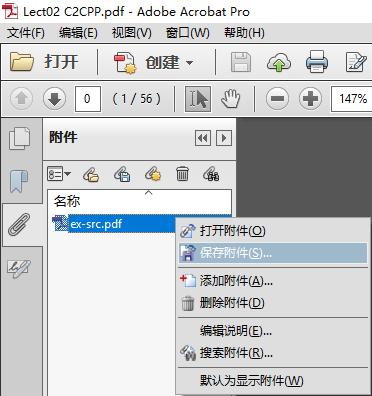
\includegraphics[height=0.35\textheight]{pdfattatchdownload01}\quad
    %或 \quad%
    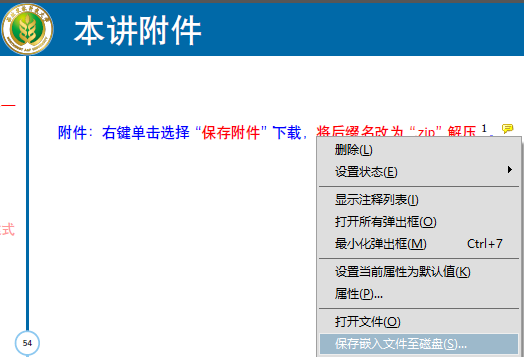
\includegraphics[height=0.35\textheight]{pdfattatchdownload02}\\[2ex]%
    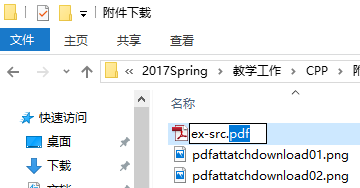
\includegraphics[height=0.255\textheight]{pdfattatchdownload03}\quad
    %$\Rightarrow$ \quad%
    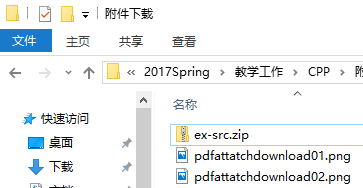
\includegraphics[height=0.255\textheight]{pdfattatchdownload04}%
  \end{center}   
\end{frame}

% \tiny
% \scriptsize
% \footnotesize
% \small
% \normalsize
% \large
% \Large
% \LARGE
% \huge
% \Huge


%%% Local Variables: 
%%% mode: latex
%%% TeX-master: "../main.tex"
%%% End: 
